\ranote{replace 'Ohm' with omega, and 'degrees celsius' with appropraite sign}A photoresistor is a variable resistor that reacts to light. Meaning that the more light the less Ohm the resistor exerts. The photoresistor used in this project have the part number VT90N2 and the datasheet can be found here \cite{photoresistor_sheet}. As can be seen in the datasheet this resistor have a typical resistance of 24k Ohm when at 10 lux (a lux scale can be found at \cite{lux_scale}) and when in darkness(meaning 0 lux) 500k Ohm. Response time above 1 fc\footnote{foot-candle is a light measurement unit like lux, 1 fc ~= 10.8 lux} are below 0.1 seconds. Below 1 fc the response time can increase up to 0.8 seconds. At 0 degrees celsius there can be up to about 13% variance, at 40 degrees celsius the variance can be upto 20%. While this is a high variance the variance normalizes to 0% at around 25 degrees. The photoresistor is sensitive to light below the visible range. It is below 18% sensitive to some wavelengths below 400 nm, which means ultraviolet light could affect readings. It is below 5% sensitive to light above 800 nm which means infrared light should not meaningfully affect the readings. (\ranote{loads of data points, how many graphs, if any should be included. All the data are from the datasheet}

Because the resistor is too sensitive for the purpose of this project a pulldown resistor is used \cite{pulldown_resistor}. A pulldown resistor lowers the base value, this means that we can detect higher levels of light. An example setup can be seen in \cref{arduino_photoresistor_wiring}
\begin{figure}[htbp]
  \centering
  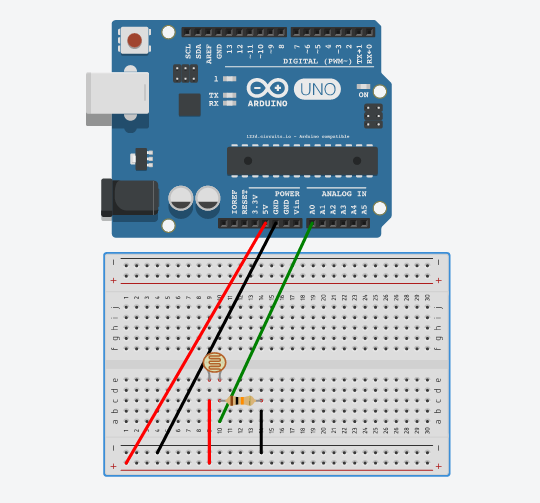
\includegraphics[width=\textwidth]{photoresistor_setup.png}
  \caption{The figure depicts wiring for a photoresistor with a pulldown resistor.}
  \label{fig:arduino_photoresistor_wiring}
\end{figure}